\documentclass{article}
\usepackage{../../typesetting/styles/report-zh}
\usepackage{threeparttable} % Add this package for tablenotes environment

\setCJKmainfont{Kaiti SC} % Main Chinese font (Songti)
\setCJKsansfont{Lantinghei TC} % Sans-serif Chinese font
% \setCJKmonofont{Maple Mono NF CN} % Monospaced Chinese font (uncomment if needed)

% Set document information
\title{周报~向嘉豪 (\today)}
\author{向嘉豪}
\date{\today}

\begin{document}

\maketitle

\begin{abstract}
  本周主要工作集中在论文图表优化及完成论文初稿方面,特别是改进了SLH-DSA签名生成流程图以增强可读性和信息传递效果。同时,完成了函数级并行(FLP)部分的实验分析及结果撰写,并完成了论文所有章节的基础初稿。
\end{abstract}

\begin{weekplan}
1) 全面检查论文中的符号一致性和潜在错误
2) 改进论文表达,提升学术写作风格
3) 进一步优化关键图表和实验结果呈现方式
\end{weekplan}

\section{论文写作}

\subsection{架构图优化}
本周主要完成了对SLH-DSA签名生成流程图的优化工作。通过对比新旧版本可以看出,新版图表采用了更为简洁明了的结构,改进了视觉层次和元素间关系的表达方式。图\ref{fig:flow_comparison}展示了此次改进的对比效果。

\begin{figure}[htb]
\centering
\begin{tabular}{cc}
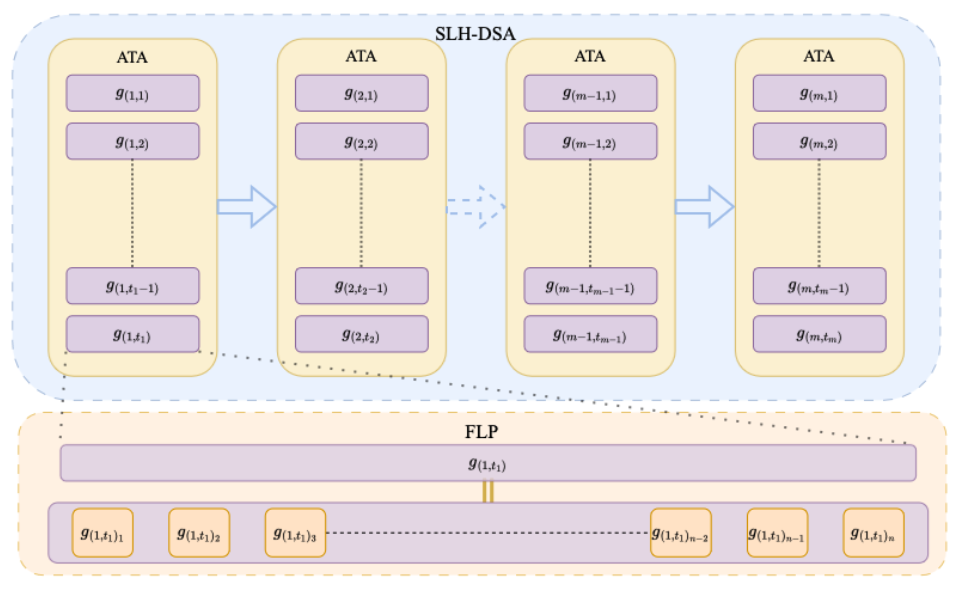
\includegraphics[width=0.48\textwidth]{fig/arch_old.png} &
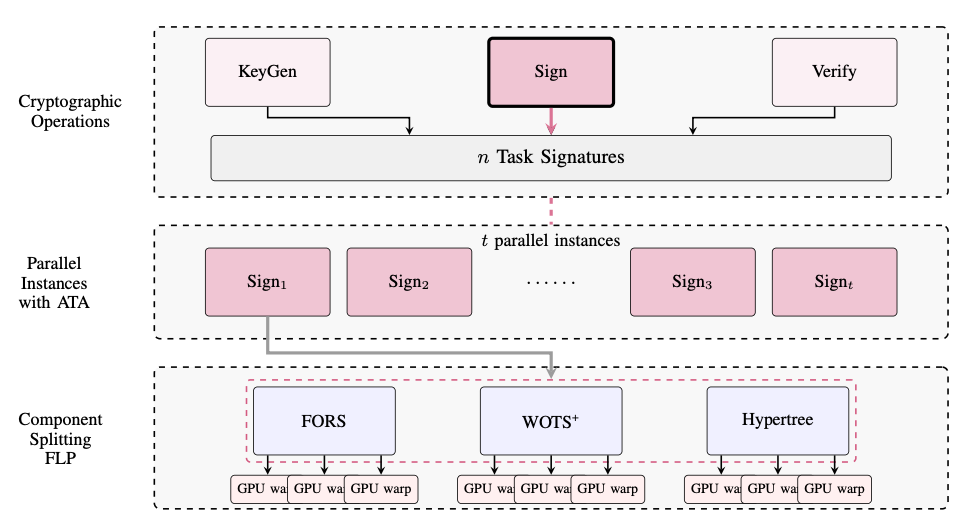
\includegraphics[width=0.48\textwidth]{fig/arch.png} \\
(a) 原始SLH-DSA签名流程图 & (b) 改进后的SLH-DSA签名流程图
\end{tabular}
\caption{SLH-DSA签名生成流程图的改进对比。左图为原始版本,右图为改进版本。新版本(b)通过优化布局和视觉元素,更清晰地展示了ATA和FLP之间关系。}
\label{fig:flow_comparison}
\end{figure}

通过此次图表优化,能够更有效地向读者传达SLH-DSA签名算法并行架构的核心流程,使论文中关键技术点的表述更加清晰。

\subsection{FLP写作和实验}

本周对论文的\red{函数级并行}(Function-Level Parallelism,\red{FLP})部分进行了深入撰写和实验分析。FLP是我们提出的\blue{Thread-Adaptive架构}中的重要组成部分,\green{有效降低了加密延迟}。

函数级并行主要围绕三种关键策略展开:\blue{(1) WOTS\textsuperscript{+}并行化},实现$l$个独立哈希链的并发计算;\blue{(2) FORS并行化},支持$k \times 2^a$个密钥元素的并行生成;以及\blue{(3) Hypertree并行化},实现跨$d$层的多Merkle树并发构建。这些技术结合了合并内存访问模式和共享内存的战略性利用。

针对FLP的有效性评估,本周完成了签名过程中组件级延迟分析实验。表\ref{tab:flp_impact}呈现了SPHINCS\textsuperscript{+}-128f参数集下各组件的延迟分布情况。

\begin{table}[h]
\centering
\caption{签名操作延迟分布 (SPHINCS\textsuperscript{+}-128f)}
\label{tab:flp_impact}
\begin{tabular}{lcc}
\hline
\textbf{组件} & \textbf{延迟 (ms)} & \textbf{占总时间百分比} \\
\hline
WOTS\textsuperscript{+} Sign & 1.857 & 0.35\% \\
FORS Sign & 29.371 & 5.58\% \\
Hypertree Sign & \red{495.252} & \red{94.07\%} \\
\hline
总签名延迟 & 526.48 & 100.00\% \\
\hline
\end{tabular}
\end{table}

实验结果表明,尽管应用了FLP优化,\red{Hypertree构建仍然占据签名延迟的主导地位(94.07\%)}。这一现象源于Hypertree中固有的顺序依赖性及其操作量,即使在组件级优化后,也限制了可实现的并行度。该发现为未来的性能增强指明了方向,\green{强调了针对Hypertree结构进行专门优化的必要性}。

本周已完成论文所有主要部分的基础初稿,包括引言、预备知识、实现方法、性能评估及结论等章节。初步形成了完整的论文框架,为后续细化工作奠定了基础。

% Replace standard bibliography commands with conditional version
\printbibliographyifcited[alpha]{../../paper}

\end{document}
